\documentclass[12pt]{article}

\title{CVWO Assignment}
\author{Tan Wei Liang}

\usepackage{graphicx}
\graphicspath{{img/}}

\usepackage{amsmath}

\usepackage{geometry}
\geometry{a4paper, portrait, margin=0.5in}

\usepackage{hyperref}
\hypersetup{
    colorlinks=true,
    linkcolor=blue,
    filecolor=magenta,      
    urlcolor=cyan,
}
\urlstyle{same}

\begin{document}
  \section{User Manual}
    \subsection{Setup}
	The app can be viewed at \href{https://cvwoassignment.herokuapp.com/}{\texttt{https://cvwoassignment.herokuapp.com/}}. If Docker is installed locally, it is also possible to set up a local instance with \texttt{sudo ./docker-init.sh}, and run it thereafter (on port 80) with \texttt{sudo ./docker-launch.sh} or just \texttt{sudo docker-compose up}.
	\subsection{Home Page}
 	A simple landing page to greet the user. Click the button to reach the Main Task List.
	
   	\begin{figure}[h]
	  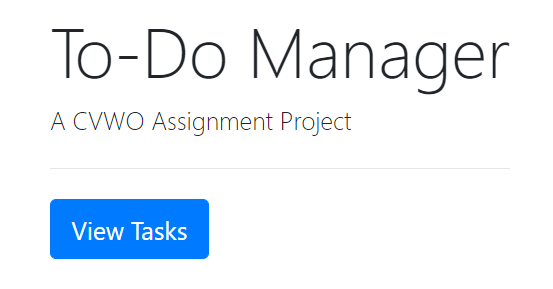
\includegraphics[width=6cm]{welcome.png}
	  \centering
	  \caption{Welcome Page}
	\end{figure}
	
    \subsection{Main Task List}
    Displays all the user's tasks. Completed tasks are hidden by default.
	  \subsubsection{Filters}
    	Some filters are available to allow the user to easily access specific tasks.
    	\begin{figure}[h]
		  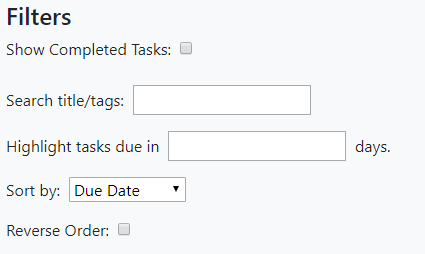
\includegraphics[width=8cm]{filters.png}
		  \centering
		  \caption{Filters}
		\end{figure}
    	\paragraph{Show Completed Tasks}
    	Enables/disables the display of completed tasks.
	   	\paragraph{Search Title/Tags}
	   	The search string is broken into tokens using whitespace as the delimiter.
	   	A task is returned as a search result if and only if ALL search tokens match (partially or fully) ANY of the title words or tags of the task.
	   	\paragraph{Highlight Tasks}
	   	Allows the user to highlight tasks that are due soon (within X days).	   	
	   	\paragraph{Sorting}
	   	The list can be sorted by due date (earliest first), title (lexicographical order, case insensitive), date created (oldest first), and \% time left ($\frac{\text{time from now to due date}}{\text{time from date created to due date}} \times 100\%$, lowest \% first). An option is available to invert the sorting order.
  	
  	  \subsubsection{Task Display}
  	    This is a table listing of the tasks after the above filters have been applied.
  	    \paragraph{Create New Task}
  	    Redirects to the new task creation page.
	  	\paragraph{Action}
	  	Each task entry has a set of action buttons to either mark as completed, view, edit, or delete the task. The user will be redirected to the relevant page on click.
    	\begin{figure}[h]
		  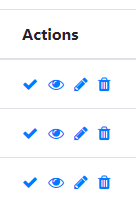
\includegraphics[width=4cm]{action.png}
		  \centering
		  \caption{Action Buttons (Complete, View, Edit, Delete)}
		\end{figure}
  	\subsection{Create New Task}
  	Displays a form for the user to create new tasks. Title and due date are mandatory fields, while description and tags are optional. When the form is submitted, the user is redirected to the task details of the newly created task.
  	\subsection{View Task Details}
  	Displays the full details of an individual task item, including the title, description, due date, tags, and completion status. Buttons are available to return to the task list, mark the task as completed, edit the task details, or permanently delete the task.
  	
   	\begin{figure}[h]
	  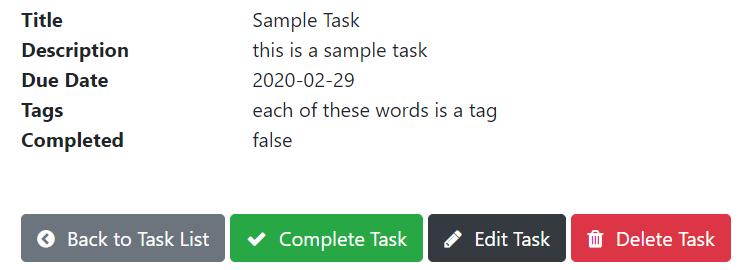
\includegraphics[width=12cm]{details.png}
	  \centering
	  \caption{Sample Task Details}
	\end{figure}
    
  \newpage
  \section{Reflection}
\setlength{\parindent}{0pt}
\setlength{\parskip}{1em}
	
	\subsection{Obstacles Faced}
	  I have spent more time than I'd like to admit working on hosting the app. Although Heroku was recommended for this assignment, I went to explore other popular hosting services such as AWS and Microsoft Azure. Furthermore, hosting seemed quite closely related to the concept of Docker containerization, so I thought that it would be an easy extension to add Docker into the hosting services.
	  
	  However, it turned out to be a lot more difficult than originally expected. Although I could get Docker and Azure working independently, I simply could not figure out how to combine them into a working cloud application. Eventually I had to cut my losses and settle for hosting via Heroku.
	
	\subsection{Learning Points}
	Through this assignment I have definitely gained some insight into web development, as I have not had much experience with it in general (especially using modern frameworks such as React). Previously, my only experience with dynamic content loading was limited to JSP and PHP. I have also taken the opportunity to learn some additional skills on top of what the assignment requires, such as \LaTeX{} (which this document is written in) and Bootstrap (for styling).
	
	The assignment mentions things like "we recommend using X as it is used by CVWO projects". Having complied with most (if not all) of these recommendations, I am able to say that I am now more prepared to take on the challenges of CVWO over the summer.
	
	As such, I would like to thank the CVWO team for coming up with this assignment, which is a good preparation for what is to come.
	
\end{document}